% v2-acmsmall-sample.tex, dated March 6 2012
% This is a sample file for ACM small trim journals
%
% Compilation using 'acmsmall.cls' - version 1.3 (March 2012), Aptara Inc.
% (c) 2010 Association for Computing Machinery (ACM)
%
% Questions/Suggestions/Feedback should be addressed to => "acmtexsupport@aptaracorp.com".
% Users can also go through the FAQs available on the journal's submission webpage.
%
% Steps to compile: latex, bibtex, latex latex
%
% For tracking purposes => this is v1.3 - March 2012

\documentclass[prodmode,acmtecs]{acmsmall} % Aptara syntax

% Package to generate and customize Algorithm as per ACM style
\usepackage[ruled]{algorithm2e}
\renewcommand{\algorithmcfname}{ALGORITHM}
\SetAlFnt{\small}
\SetAlCapFnt{\small}
\SetAlCapNameFnt{\small}
\SetAlCapHSkip{0pt}
\IncMargin{-\parindent}

\usepackage[english]{babel}
\usepackage{tikz}
\usetikzlibrary{positioning}
\usepackage[pass]{geometry}
\usepackage{graphicx}
\usepackage{epsfig}
\usepackage{url}
\usepackage{color}
\definecolor{nodecolor}{RGB}{202,202,202}
\newlength\framesep
\setlength\framesep{16pt}
\pgfdeclarelayer{background}
\pgfsetlayers{background,main}
\pgfkeys{
	/tikz/node distance/.append code={
		\pgfkeyssetvalue{/tikz/node distance value}{#1}
	}
}

\widowpenalty=10000
\clubpenalty=10000

% Metadata Information
\acmVolume{9}
\acmNumber{4}
\acmArticle{39}
\acmYear{2010}
\acmMonth{3}

% Copyright
%\setcopyright{acmcopyright}
%\setcopyright{acmlicensed}
%\setcopyright{rightsretained}
%\setcopyright{usgov}
%\setcopyright{usgovmixed}
%\setcopyright{cagov}
%\setcopyright{cagovmixed}

% DOI
\doi{0000001.0000001}

%ISSN
\issn{1234-56789}

% Document starts
\begin{document}

% Page heads
\markboth{G. Zhou et al.}{A Multifrequency MAC Specially Designed for WSN Applications}

% Title portion
\title{Total Platform Cyber Protection}

%TODO Adam: Not sure if anon submission so just leaving like this for now
\author{
%First Author
%\affil{Arizona State University}
%Second Author
%\affil{Arizona State University}
%Third Author
%\affil{Arizona State University}
%Fourth Author
%\affil{Arizona State University}
%Fifth Author
%\affil{Arizona State University}
%Sixth Author
%\affil{Arizona State University}
%Seventh Author
%\affil{Arizona State University}
}
% NOTE! Affiliations placed here should be for the institution where the
%       BULK of the research was done. If the author has gone to a new
%       institution, before publication, the (above) affiliation should NOT be changed.
%       The authors 'current' address may be given in the "Author's addresses:" block (below).
%       So for example, Mr. Abdelzaher, the bulk of the research was done at UIUC, and he is
%       currently affiliated with NASA.

% TODO Sai: Discuss story with yeganeh and get a nice little abstract here
\begin{abstract}
Multifrequency media access control has been well understood in
general wireless ad hoc networks, while in wireless sensor networks,
researchers still focus on single frequency solutions. In wireless
sensor networks, each device is typically equipped with a single
radio transceiver and applications adopt much smaller packet sizes
compared to those in general wireless ad hoc networks. Hence, the
multifrequency MAC protocols proposed for general wireless ad hoc
networks are not suitable for wireless sensor network applications,
which we further demonstrate through our simulation experiments. In
this article, we propose MMSN, which takes advantage of
multifrequency availability while, at the same time, takes into
consideration the restrictions of wireless sensor networks. Through
extensive experiments, MMSN exhibits the prominent ability to utilize
parallel transmissions among neighboring nodes. When multiple physical
frequencies are available, it also achieves increased energy
efficiency, demonstrating the ability to work against radio
interference and the tolerance to a wide range of measured time
synchronization errors.
\end{abstract}


%
% The code below should be generated by the tool at
% http://dl.acm.org/ccs.cfm
% Please copy and paste the code instead of the example below. 
%
\begin{CCSXML}
	<ccs2012>
	<concept>
	<concept_id>10002978.10003001.10010777</concept_id>
	<concept_desc>Security and privacy~Hardware attacks and countermeasures</concept_desc>
	<concept_significance>400</concept_significance>
	</concept>
	<concept>
	<concept_id>10002978.10003001.10003003</concept_id>
	<concept_desc>Security and privacy~Embedded systems security</concept_desc>
	<concept_significance>400</concept_significance>
	</concept>
	<concept>
	<concept_id>10002978.10003006.10003007</concept_id>
	<concept_desc>Security and privacy~Operating systems security</concept_desc>
	<concept_significance>400</concept_significance>
	</concept>
	<concept>
	<concept_id>10002978.10003022</concept_id>
	<concept_desc>Security and privacy~Software and application security</concept_desc>
	<concept_significance>400</concept_significance>
	</concept>
	</ccs2012>
\end{CCSXML}

\ccsdesc[400]{Security and privacy~Hardware attacks and countermeasures}
\ccsdesc[400]{Security and privacy~Embedded systems security}
\ccsdesc[400]{Security and privacy~Operating systems security}
\ccsdesc[400]{Security and privacy~Software and application security}
%
% End generated code
%

% We no longer use \terms command
%\terms{Design, Algorithms, Performance}

%TODO Sai: Add keywords here
\keywords{}

\acmformat{Gang Zhou, Yafeng Wu, Ting Yan, Tian He, Chengdu Huang, John A. Stankovic,
and Tarek F. Abdelzaher, 2010. A multifrequency MAC specially
designed for  wireless sensor network applications.}
% At a minimum you need to supply the author names, year and a title.
% IMPORTANT:
% Full first names whenever they are known, surname last, followed by a period.
% In the case of two authors, 'and' is placed between them.
% In the case of three or more authors, the serial comma is used, that is, all author names
% except the last one but including the penultimate author's name are followed by a comma,
% and then 'and' is placed before the final author's name.
% If only first and middle initials are known, then each initial
% is followed by a period and they are separated by a space.
% The remaining information (journal title, volume, article number, date, etc.) is 'auto-generated'.

\begin{bottomstuff}
This work is supported by the National Science Foundation, under
grant CNS-0435060, grant CCR-0325197 and grant EN-CS-0329609.

Author's addresses: G. Zhou, Computer Science Department,
College of William and Mary; Y. Wu  {and} J. A. Stankovic,
Computer Science Department, University of Virginia; T. Yan,
Eaton Innovation Center; T. He, Computer Science Department,
University of Minnesota; C. Huang, Google; T. F. Abdelzaher,
(Current address) NASA Ames Research Center, Moffett Field, California 94035.
\end{bottomstuff}

\maketitle

\section{Introduction}
Traditional security defenses for the computing environment have
focused on securing the \emph{border} of the network, as this is the
entry place for most attackers. However, even with sophisticated
border technologies in place, there are constant attacks and data
breaches against our networks. The goal of this work is to survey the
state of security for the entire computing platform, in order to
identify specific areas that are underserved by the research community
and that require additional research and investment.

Modern computing infrastructure serves a wide array of needs, with
diverse technologies and implementations: embedded systems, cloud
computing, sensor networks, desktops, mobile devices, and industrial
control systems. Rather than consider each of these computing
platforms independently, in this work we abstracted the computing
platform into several layers, each of which are applicable to every
computing infrastructure. In particular, we analyzed the security
research performed at the following layers of the computing platform:
hardware, firmware, bus, hypervisor, operating system, application,
and network layers (Figure~1).

The goal of this work is to focus research effort on \emph{securing
	the entire computing platform.} An attack must effectively target a
specific vulnerability in a specific layer of the computing stack, and
an attacker uses that vulnerability to establish persistence on the
machine, potentially attacking the underlying computing layers of the
same machine or leveraging their place in the network to attack other
machines. Therefore, if we wish to increase the security of our
computing systems, and reduce the number and scope of security
breaches, it is essential that we encourage focus on novel ideas,
algorithms, and techniques to secure every level of the computing
stack.

In this report, we will first discuss the computing stack, and, for
every layer, we will describe the layer, identify primary threats
against the layer, and summarize the research on attempts to secure
that layer, and finally we will determine areas that require further
research investment to ensure the security of the layer.\begin{figure}
\centering
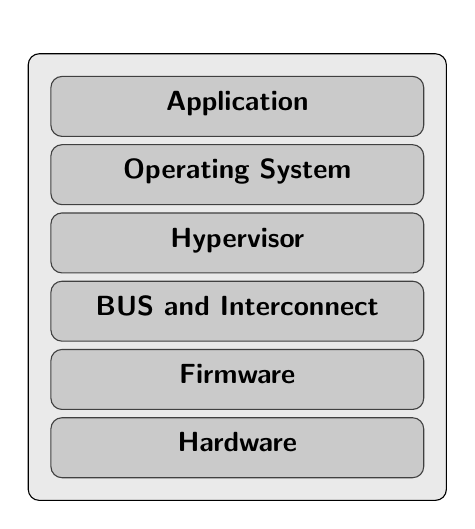
\begin{tikzpicture}[scale=0.50,node distance=3pt,outer sep=0pt,
platformlayer/.style={
  draw=darkgray,
  fill=nodecolor,
  rounded corners,
  text width=4.5cm,
  font={\sffamily\bfseries\color{black}},
  align=center,
  text height=9pt,
  text depth=6pt},
]
\node[platformlayer] (APP) {Application};
\node[platformlayer,below=of APP](OS) {Operating System};
\node[platformlayer,below=of OS] (HYP) {Hypervisor};
\node[platformlayer,below=of HYP](BUS){BUS and Interconnect};
\node[platformlayer,below=of BUS](FW) {Firmware};
\node[platformlayer,below=of FW](HW) {Hardware};

\begin{pgfonlayer}{background}
\draw[platformlayer,draw=black,fill=nodecolor!40]([xshift=-\framesep,yshift=1\framesep]current bounding box.north west)
rectangle ([xshift=\framesep,yshift=-\framesep]current bounding box.south east) 
node[below] at (0,2) {};

\end{pgfonlayer}
\end{tikzpicture}
\caption{Computing Platform Layers}
\label{fig:layers}
\end{figure}

\section{Background}
Here, we consider the diverse array of computing platforms as a number
of abstracted layers: hardware, firmware, bus, hypervisor, operating
system, application, and network layers. In this way, we can
categorize the research efforts that target each layer.

The layers are arranged from lowest to highest layer. The lower layer
has more control over the computing system, while the upper layers
have less control. For instance, the Hardware layer has total control
over the physical hardware and memory of the machine, while an
application running in the Application layer can only see a portion of
the machine's memory (because of the virtual memory used by the
Operating System).

A typical compromise, in relation to the proposed layers, is the
following: A vulnerability in an application is targeted, thus
allowing the attacker full control of the application layer. From
here, the attacker can scan the other applications on the network and
attempt to exploit those applications, thus spreading horizontally
throughout the network. Alternatively, as the application layer is the
least privileged and least persistent of the layers, the attack can
attempt to further the compromise on the lower layers of the machine.
For instance, the attacker can exploit the hypervisor layer to
compromise the host hypervisor. From this vantage point, the attacker
can transparently extract information from all the other guest
Operating Systems. More insidiously, the attacker can even exploit the
firmware level, which allows the attacker to persist even after
a complete reinstall of the operating system.

In our abstract model, the lower levels have more control over the
computing system, yet they have a smaller attacker surface. However,
the lower levels can be attacked by exploiting the upper levels. Also, the upper
levels trust the abstractions provided by the lower levels. For
instance, the application-layer visualization of an industrial control
system trusts that the data reported by the hardware layer is
accurate. If an attacker is able to control and manipulate the
hardware to falsely report the state of the system, the entire
integrity of the system can be compromised.

The interconnected nature of the layers means that the security of the
entire layer must be a priority. However, at the same time, the
security improvement of any layer will have an amplifying effect on
the security of the whole system. For instance, improvement to the
security of the application layer decreases the chance of an
application compromise, which further decreases the risk of the attack
propagating throughout the network and through the other layers.

\section{Hardware}

Hardware underpins all of modern computing. While most software is
constructed and written in such a way as to abstract the
peculiarities of the underlying hardware, the software cannot
execute without hardware. In our abstracted model of the computing
stack, hardware is at the bottom, which means that it has complete
control of the computing system.

For hardware here, we consider all types of hardware in the computing
system: CPUs, SoCs, or any other integrated circuit (IC) that performs
computation or communication on behalf of the upper computing layers.
This also includes networking cards and other peripheral devices
(Bluetooth or USB devices), which may have their own special purpose
embedded hardware.

A key difficulty in analyzing the security concerns of hardware is
reverse engineering the workings of the hardware. Traditional
techniques to reverse engineer hardware require destroying the chip,
and if a single hardware component is destroyed to reverse engineer,
there is no guarantee that other hardware is identical to the reverse
engineered chip.

\subsection{Threats}

As the lower-most level of the computing stack, all layers implicitly
trust that the hardware is executing correctly. Therefore, if an
adversary is able to maliciously control the hardware execution, they
can compromise all layers of the computing stack. Thus, the security
of the hardware is of paramount importance.

The main threat considered by the literature on hardware is the threat
of Trojan logic. This is malicious logic that is introduced into the
% adversary, by definition is a malicious entity.
hardware chip by an adversary. Trojan introduction can be
done at several points of the hardware lifecycle:

\begin{itemize}
	
	\item \textbf{Design}. A malicious insider can incorporate a Trojan into the
	design of the hardware.
	
	\item \textbf{Third-party IP}. Oftentimes, hardware designers will take
	advantage of the functionality of third-party components, using them
	as a black-box. Thus, a third-party can include malicious Trojan
	logic.
	
	\item \textbf{Compilation of Design}. When the design of the hardware is
	compiled, but before it is sent for fabrication, the design could be
	changed to incorporate the Trojan logic. Note that this differs from
	Design-time, because the Trojan logic is not included in the design.
	Consider the case of malware on a hardware designer's machine, which
	changes the design when it is compiled.
	
	\item \textbf{Manufacture}. A malicious manufacturer can introduce Trojan logic into hardware after the design is received but before the hardware
	is fabricated.
	
	\item \textbf{Delivery}. A malicious hardware component containing Trojan logic can be swapped with a benign component after fabrication but before
	delivery and installation.
	
\end{itemize}

The malicious Trojan logic behavior comes in three different forms:
% TODO: Sai: is this three or two??

\begin{itemize}
	
	\item \textbf{Trigger-based}. The malicious behavior or logic is only expressed when certain conditions are met. Consider a Trojan logic in a CPU,
	which changes the executing code to Ring 0 (with the most
	privileges) when a specific sequence of instructions are issued. The
	trigger can be internal to the chip, such as in the CPU case, or
	could be external, for instance a certain radio frequency will
	trigger the malicious code.
	
	\item \textbf{Constant}. The malicious behavior or logic is continually
	executed and subtly changes the output of the hardware in a way that
	compromises security. Consider a Trojan logic of a Wi-Fi card, which
	leaks the Wi-Fi passphrase by embedding it in the operating
	parameters of the Wi-Fi radio.
	
\end{itemize}

These features of Trojan logic in hardware drive the research that
attempts to detect them. 

\subsection{Research}

Most research into hardware Trojans deal with using side-channel
analysis to identify the malicious Trojan behavior~\cite{lee2005,
agrawal2007, banga2008, banga2008a, jin2008, du2010, narasimhan2011,
narasimhan2012, cao2013, davoodi2013, dworak2013, forte2013,
liu2013, liu2014, bao2015}. This research uses power analysis, heat
analysis, or other side-effects to determine that the hardware is
executing abnormal logic. Unfortunately, this typically requires
building a model based on a ``golden'' or known-good hardware, which
is often not accessible. Furthermore, as chips become more complex,
the Trojan logic become an increasingly smaller portion of the chip,
which in turn reduces the side-channel behavior of the chip
significantly. 

Other research has demonstrated the attacks that are possible by
actually implementing Trojan behavior~\cite{king2008, jin2010,
sturton2011, liu2013, jin2014, zhang2014}. This line of research
shows that Trojan logic is feasible for an attack.

Of particular practical interest is a description of \emph{actual
Trojan logic} discovered in the ProASIC3 Flash FPGA military
chip~\cite{skorobogatov2012}. While in this case it was not proved
that the logic introduced to the chip was intentionally malicious,
nevertheless there existed functionality in the hardware that was
explicitly denied by the hardware designer. 

Another avenue of research is to change the design of the chip itself,
in order to improve the testability of the chip or to increase the
effectiveness of the side-channel analysis~\cite{chakraborty2008,
li2008, salmani2009, hicks2010, rosenfeld2011, waksman2011,
bhunia2013, davoodi2013, rajendran2013, rolt2014}. This line of
research attempts to rethink designing the hardware itself. However, a
major drawback is that this can increase the cost of the hardware and
it must be somehow mandated to be used in COTS components. 

JTAG is a main avenue of reverse engineering hardware, so some work
has investigated the problem of securing JTAG access to
hardware~\cite{rosenfeld2010, ren2015}. The main idea is to allow only
authenticated users to have access to the JTAG functionality, however
this increases the cost and complexity of implemented JTAG. 

Another approach is to change the design of the chip to support
runtime monitoring~\cite{waksman2010}. In this way, the hardware
is monitoring itself, 
rather than external analysis of
side-channels. However, this has all the same drawbacks of changing
the design of hardware, in addition to not being robust in the face of
a powerful attacker who is able to alter the design. 

Recent approaches suggest to use machine-learning techniques to
identify the Trojan logic~\cite{haider2015}. Another approach attempts
to use a formal verification technique in order to prove that no
malicious logic was added to the hardware~\cite{guo2015}.

Finally, there are several surveys conducted on hardware security,
which provide a good overview of the field~\cite{wang2008,
tehranipoor2010, guin2014, guin2014a, guin2014b}.

Important problems include how to deal with counterfeit chips, better
non-destructive examination methods, continuous monitoring of the
integrity not just at boot time, and detection of backdoors and 
``undocumented features''.  Hardware design can also be done to
aid this process, e.g., having some part of the chip consume more power
to make it more identifiable for authentication purposes.  Other
possibilities include running multiple chips with different
implementations side-by-side and comparing results to detect unexpected
behavior.

\subsection{Suggested Focus Areas}

A key problem with hardware security is non-destructive IC
examination, identification, and authentication - how to ensure that
the chip that is designed is what is actually fabricated, with no
additional logic.

An additional neglected area is how to detect malicious Trojan logic
in third-party components. This would require some type of static
analysis or simulated dynamic analysis of third-party components,
which could detect Trojan logic.

Another approach that could be effective is how to properly test the
functionality of hardware after it has been fabricated. This could
include changing the design of the chip to allow better/more guided
fuzz testing of the chip itself, in order to discover the Trojan
logic.

Finally, a prevention approach could be taken, to monitoring the upper
layers of the computing stack for attempts to exploit the underlying
hardware. This can also include changing or altering the firmware
layer in such a way that it is not possible to exercise the Trojan
logic, potentially using randomization techniques similar to ASLR. 

\section{Firmware}

%Note: I did not remove the previous versions of those paragraphs
%(commented them) so feel free to check the previous versions and 
%revert them if my changes have problems.

%Firmware is the layer of software that sits and interacts directly
%with the hardware. Typically, the firmware is controlled from the
%upper layers by device drivers in the Operating System.

%Faris:
Firmware is the layer of software that sits and interacts directly
with the hardware. Typically, the firmware is controlled by the
device drivers in the upper layers of the Operating System.

%Many different hardware contain firmware, for instance the boot BIOS
%on a motherboard is a form of firmware, embedded systems often contain
%specific firmware, hardware peripherals such as network cards contain
%firmware as well. We consider all such areas as firmware.

%Faris:
Many different hardware contain firmware. For instance: the boot BIOS
on a motherboard, embedded systems that contain
specific firmware, hardware peripherals such as network cards. 
We consider all such areas as firmware.

%The key traits of firmware is that, although it is binary code, it is
%operating/interacting directly with the hardware, so there are no
%%OS-style abstraction layers such as virtual memory, well-defined
%system calls, or hardware abstraction. Therefore, each firmware is
%binary code which is specifically tailored to a specific hardware
%platform.

%Faris:
Although firmware is binary code, it is
operating/interacting directly with the hardware, so there are no
OS-style abstraction layers such as virtual memory, well-defined
system calls, or hardware abstraction which is the key trait of firmware. 
Therefore, each firmware is specifically tailored to a specific hardware platform.

%Due to the hardware-specific nature of firmware, \emph{reverse
%	engineering} is critical to understanding the firmware. In addition,
%reverse engineering is particularly challenging because source code is
%frequently unavailable, and vendors' desire to protect their
%intellectual property makes them actively obfuscate their
%firmware. All this means that, extracting semantically useful
%information from firmware is a key first step to performing any
%security analysis of the firmware.

%Faris:
Due to the hardware-specific nature of firmware, \emph{reverse
	engineering} is critical to understand it. In addition,
reverse engineering is particularly challenging because the source code is
frequently unavailable, and vendors' desire to protect their
intellectual property makes them actively obfuscate their
firmware. This means, extracting semantically useful
information from firmware is the first and key step to perform any
security analysis of the firmware.

\subsection{Threats}

As the lowest-level of software code in the computing stack, threats
to firmware can compromise the security of the entire machine.
Firmware security is concerned with two main threats: (1)
vulnerabilities in the firmware code itself which allow an attacker to
execute arbitrary code with the capabilities of the firmware and (2)
firmware with intentional Trojan (backdoor) capabilities.

%Vulnerabilities in the firmware code allow an attacker to execute
%arbitrary code with the permissions of the firmware. The class of
%vulnerabilities are not unique to firmware, as they are the same class
%of vulnerabilities that infect traditional binary software (buffer
%overflows, logic flaws, etc.). However, firmware typically has full
%control over the entire computing system, therefore vulnerabilities in
%firmware are much more severe than those in the application layer. In
%addition, if an attacker is able to persist their exploit --- because the
%compromise occurs at such a low layer of the computing system --- the
%attacker can persist \emph{even after reinstalling the operating
%	system or application}.

%Faris:
Vulnerabilities in the firmware code allow an attacker to execute
arbitrary code with the permissions of the firmware. The class of
vulnerabilities are not unique to firmware, as they are the same class
of vulnerabilities that infect traditional binary software (buffer
overflows, logic flaws, etc.). However, firmware typically has full
control over the entire computing system, therefore vulnerabilities in
firmware are much more severe than those in the application layer. In
addition, the attacker may remain in the system because the
compromise occurs at such a low layer of the computing system so the
exploit persists \emph{even after reinstalling the operating
	system or application}.

%The attack surface for firmware varies depending on where it is used.
%In the most general case, the attacks can come from the upper layers,
%specifically the Operating System or Hypervisor layers, as these are
%the layers of the computing stack that can directly communicate with the
%firmware. However, other firmware can be attacked either directly
%through the Hardware layer itself, or through the data being
%transmitted through the firmware from the hardware. For instance, a
%network card firmware could be attacked through network traffic that
%the firmware processes.

%Faris:
The attack surface for firmware varies depending on where it is used.
In the general case, the attacks can come from the upper layers,
specifically the Operating System or Hypervisor layers, as these are
the layers of the computing stack that can directly communicate with the
firmware. However, other firmware can be attacked either directly
through the Hardware layer, or through the data being
transmitted through the firmware from the hardware. For instance, a
network card firmware could be attacked through network traffic that
the firmware processes.

Traditional vulnerability analysis is not effective on firmware, due
to the specificity of the firmware for the specific hardware and the
lack of a well-defined operating system abstraction for the firmware
code. In essence, each firmware is a custom binary with little in the
way of assumptions that vulnerability analysis can take advantage of. 

%Trojan capabilities in the firmware itself can allow a system to be
%remotely controlled or accessed. This is similar to a vulnerability,
%in that an attacker is able to control the firmware, however the key
%difference lies in the fact that Trojan behavior will be intentionally
%obfuscated by an attacker, whereas a vulnerability is accidentally
%introduced by a benign developer. Therefore, Trojan behavior is 
%more difficult to detect, because there is an active adversary who is
%intentionally obfuscating the behavior. 

%Faris:
Trojan capabilities in the firmware can allow a system to be
remotely controlled or accessed. This is similar to a vulnerability,
in that an attacker is able to control the firmware, however the key
difference lies in the fact that Trojan behavior can be intentionally
obfuscated by an attacker, whereas a vulnerability can accidentally
introduced by a benign developer. Therefore, Trojan behavior is 
difficult to detect.

%Vulnerabilities in the firmware and Trojan capabilities are related
%because both require \emph{understanding} the behavior and semantics
%of the firmware code. This is why reverse engineering is such a
%critical component of securing the threats against the firmware layer:
%in order to detect either vulnerabilities or Trojan functionality, an
%automated tool must first understand the semantics of the particular
%firmware/hardware combination. 

%Faris:
Vulnerabilities in the firmware and Trojan capabilities are related
because both require \emph{understanding} the behavior and semantics
of the firmware code. This is why reverse engineering is such a
critical component of securing the firmware layer against the threats.
In order to detect vulnerabilities or trojan functionality, an
automated tool must understand the semantics of the particular
firmware/hardware combination. 

\subsection{Research}
%Faris: Some fixes below. 
Researchers have attempted to identify real-world attacks on firmware
code~\cite{tsow2006, cui2010, duflot2011, basnight2013, cui2013,
	zaddach2013, zaddach2013a, maskiewicz2014, stuttgen2015}. These
attacks are particularly effective, and researchers have shown that
these are able to persist through a reboot and cannot be detected by
the upper layers. 

Other approaches are about how to prevent the tampering of
firmware~\cite{adelstein2002, zhou2007, zhou2009}. These protect from
the threat of tampering or altering the firmware, however it does not
address vulnerable firmware. 

Another approach includes runtime monitoring into the
firmware, so that compromises can be detected~\cite{cui2010a,
	cui2011}. This approach is further complicated by the lack of
abstractions in the firmware environment. 

Recent work has looked into the problem of updating the design of the
firmware so that it has security features, such as memory handling and
avoiding information leakage~\cite{koeberl2014, kauer2007}. However,
forcing firmware developers to use such features is an open issue.

Very few work has looked into how to reverse engineer and understand the
firmware~\cite{zaddach2014}. This problem is of particular interest,
as understanding the semantics of the firmware and how it interacts
with hardware is a key challenge. 

Recent work has looked into how to detect vulnerabilities in
firmware~\cite{davidson2013, costin2014, shoshitaishvili2015}. One of
these has an excellent website\footnote{\url{http://firmware.re}}
that contains the results of their reverse engineering and
vulnerability analysis~\cite{costin2014}.

\subsection{Suggested Focus Areas}
%Faris: Some fixes below.
Of all the layers, firmware has received the least attention from the
research community. Therefore, we believe that focus on this research
area will yield significant dividends. 

The major challenge with preventing firmware vulnerabilities is how to decouple
firmware from the hardware, potentially using emulation of the
hardware, in order to aid the analysis of the firmware. 

In a similar vein, there is need for automated reverse engineering tools,
including analysis of memory layouts, code modules, even answering the
simple question of what is code in a firmware binary and what is data.

Finally, even if we find vulnerabilities or Trojan logic in a
firmware, there is still the unanswered question of how to patch or
update the functionality of the firmware while still guaranteeing the
behavior of the firmware. This is particularly complicated due to the
real-time requirements of the firmware and the potentially concurrent
executions.  

\section{Performance Evaluation}

During all the experiments, the Geographic Forwarding (GF)
[Akyildiz 2001] routing protocol is used. GF exploits geographic
information of nodes and conducts local data-forwarding to achieve
end-to-end routing. Our simulation is
configured according to the settings in
Table~\ref{tab:one}. Each run lasts for 2 minutes and
repeated 100 times. For each data value we present in the results,
we also give its 90\% confidence interval.
% Table
\begin{table}%
\tbl{Simulation Configuration\label{tab:one}}{%
\begin{tabular}{|l|l|}
\hline
TERRAIN{$^a$}   & (200m$\times$200m) Square\\\hline
Node Number     & 289\\\hline
Node Placement  & Uniform\\\hline
Application     & Many-to-Many/Gossip CBR Streams\\\hline
Payload Size    & 32 bytes\\\hline
Routing Layer   & GF\\\hline
MAC Layer       & CSMA/MMSN\\\hline
Radio Layer     & RADIO-ACCNOISE\\\hline
Radio Bandwidth & 250Kbps\\\hline
Radio Range     & 20m--45m\\\hline
\end{tabular}}
\begin{tabnote}%
\Note{Source:}{This is a table
sourcenote. This is a table sourcenote. This is a table
sourcenote.}
\vskip2pt
\Note{Note:}{This is a table footnote.}
\tabnoteentry{$^a$}{This is a table footnote. This is a
table footnote. This is a table footnote.}
\end{tabnote}%
\end{table}%

\section{Conclusions}

In this article, we develop the first multifrequency MAC protocol for
WSN applications in which each device adopts a
single radio transceiver. The different MAC design requirements for
WSNs and general wireless ad-hoc networks are
compared, and a complete WSN multifrequency MAC design (MMSN) is
put forth. During the MMSN design, we analyze and evaluate different
choices for frequency assignments and also discuss the nonuniform
back-off algorithms for the slotted media access design.


% Appendix
\appendix
\section*{APPENDIX}
\setcounter{section}{1}
In this appendix, we measure
the channel switching time of Micaz [CROSSBOW] sensor devices.
In our experiments, one mote alternatingly switches between Channels
11 and 12. Every time after the node switches to a channel, it sends
out a packet immediately and then changes to a new channel as soon
as the transmission is finished. We measure the
number of packets the test mote can send in 10 seconds, denoted as
$N_{1}$. In contrast, we also measure the same value of the test
mote without switching channels, denoted as $N_{2}$. We calculate
the channel-switching time $s$ as
\begin{eqnarray}%
s=\frac{10}{N_{1}}-\frac{10}{N_{2}}. \nonumber
\end{eqnarray}%
By repeating the experiments 100 times, we get the average
channel-switching time of Micaz motes: 24.3$\mu$s.

\appendixhead{ZHOU}

% Acknowledgments
\begin{acks}
The authors would like to thank Dr. Maura Turolla of Telecom
Italia for providing specifications about the application scenario.
\end{acks}

% Bibliography
\bibliographystyle{ACM-Reference-Format-Journals}
\bibliography{papers}
                             % Sample .bib file with references that match those in
                             % the 'Specifications Document (V1.5)' as well containing
                             % 'legacy' bibs and bibs with 'alternate codings'.
                             % Gerry Murray - March 2012

% History dates
\received{February 2007}{March 2009}{June 2009}

\end{document}
% End of v2-acmsmall-sample.tex (March 2012) - Gerry Murray, ACM


